\section{Results}\label{sec:results}

\subsection{Exploration of the dataset}

The full dataset comprises 1328 plot-year observations across the 6 viticultural regions of western Switzerland as shown in the map depicted in \cref{fig:map}.

\begin{figure}[tbp]
\centering
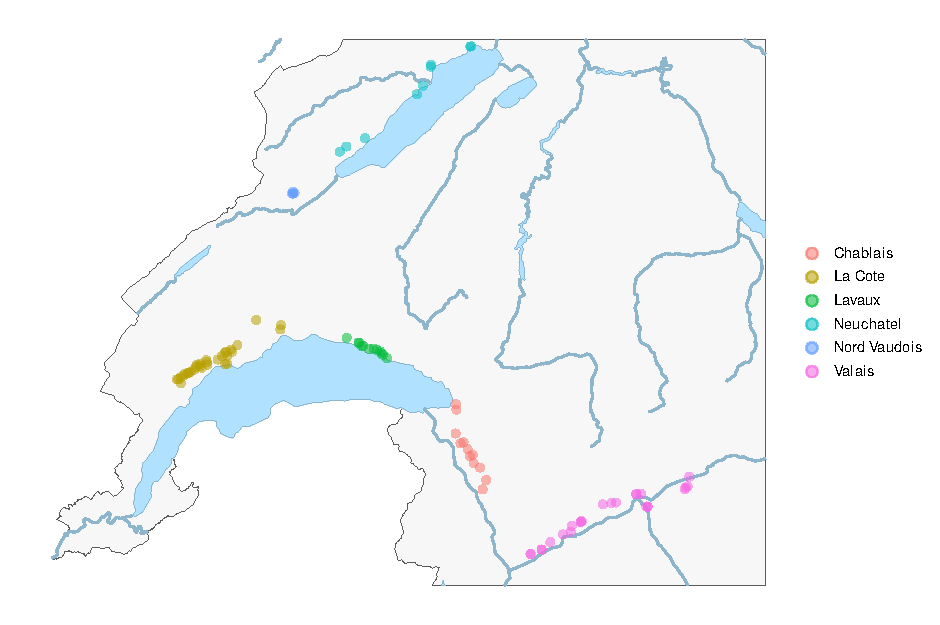
\includegraphics[width=\textwidth]{Fig1_map_plots_only.pdf}
\caption{Map of the plots used in this study. An interactive version with the locations of the meteorological stations is available in the supplementary material.}\label{fig:map}
\end{figure}

The sample composition is heavily dominated by the La Côte region. On \cref{fig:samples}b, the distribution of the samples in terms of cultivar and regions over the years is displayed. Chasselas is predominant in the cultivars, essentially because of its importance in Western Switzerland, while the La Côte region was the most sampled, because of proximity with the Changins agronomical research station.

\begin{figure}[tbp]
\centering
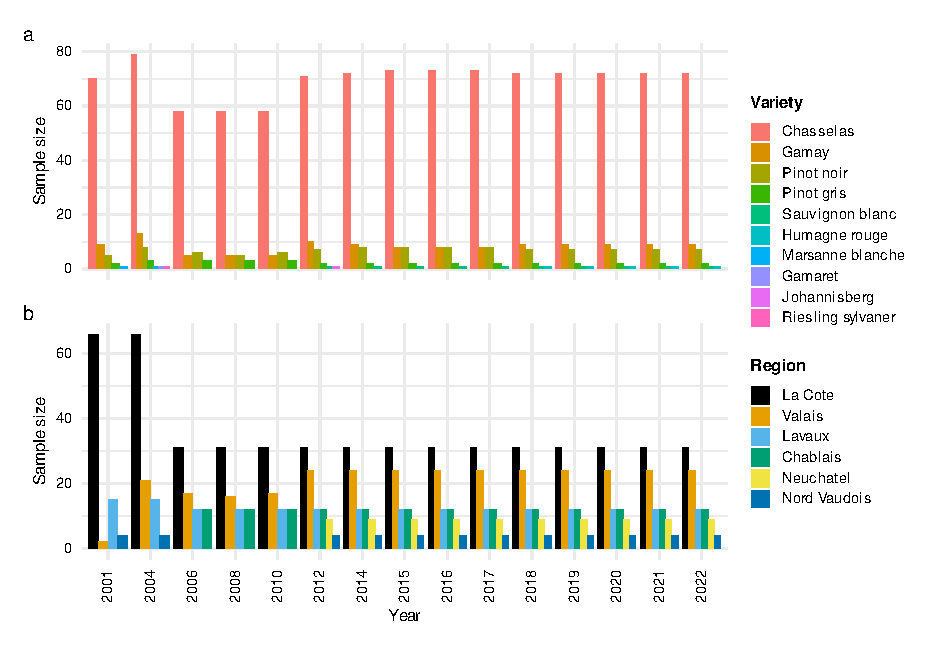
\includegraphics[width=\textwidth]{Fig2_3.pdf}
\caption{Number of plots sampled per year (a) by grape variety and (b) by viticultural region.}\label{fig:samples}
\end{figure}

\subsection{Temporal evolution of Esca expression}

The temporal evolution of the combined Esca expression (foliar symptoms + apoplexy, in \% of vine stocks) is displayed as yearly boxplots across all observed plots (\cref{fig:temporal}a). Smooth trend lines for the mean (loess) and median \citep{fasiolo_fast_2021,fasiolo_qgam_2021} are also displayed to highlight the temporal patterns. We observed a slight negative trend in the incidence of the esca disease over the years.

\begin{figure}[tbp]
\centering
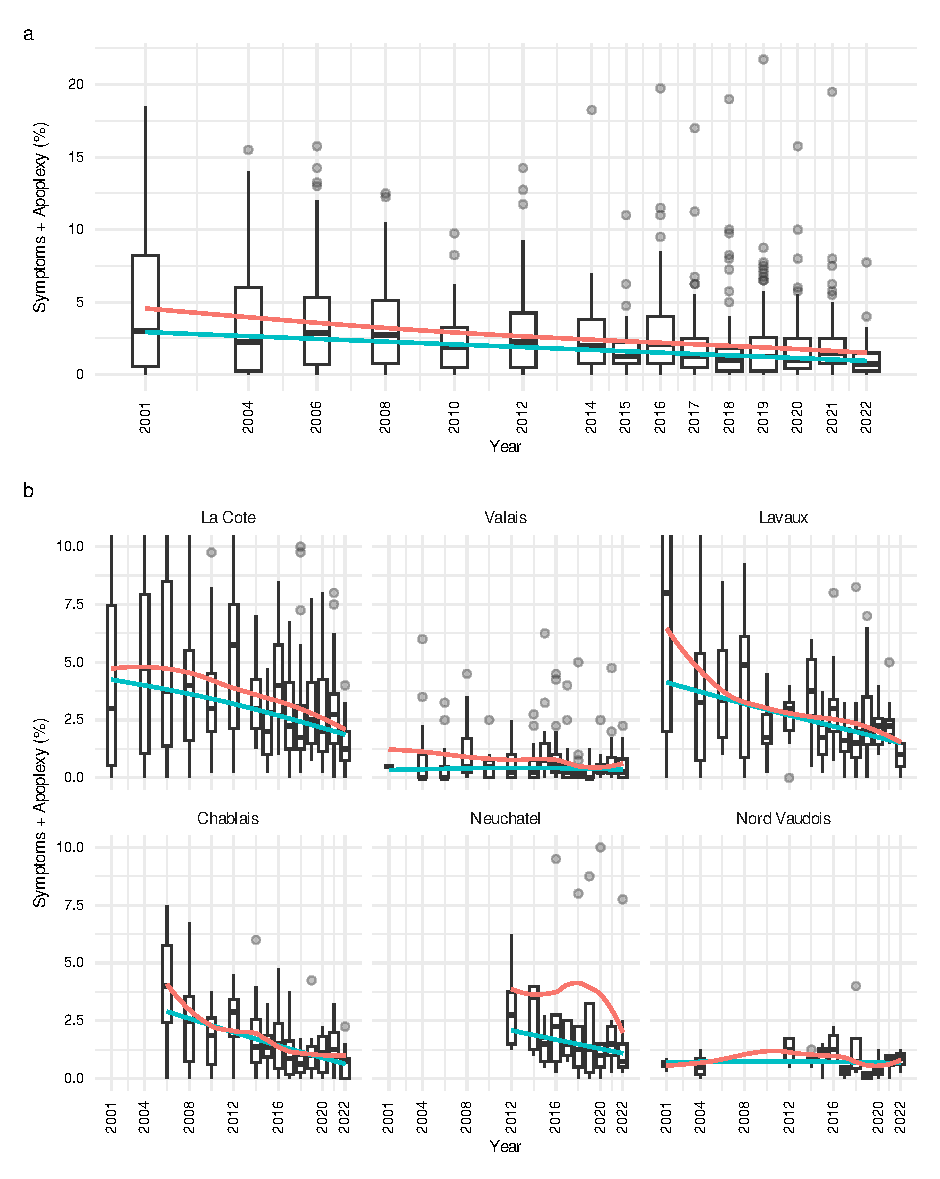
\includegraphics[width=\textwidth]{Fig4_5.pdf}
\caption{Temporal evolution of esca incidence, expressed as the percentage of vine stocks with foliar symptoms or apoplexy per plot, (a) for all plots and (b) by viticultural region. Boxplots show the distribution of plot incidences in each survey year. Red lines: smooth mean (loess); blue lines: smooth median (quantile GAM). In (b) the y axis is truncated at 10\% for readability, so some extreme values are not shown.}\label{fig:temporal}
\end{figure}

When examined by region, the same temporal boxplots reveal substantial regional disparities in Esca expression levels (\cref{fig:temporal}b). We observe a signal of a negative trend in disease expression with strong interannual variability. The negative trend is quite pronounced in regions with a higher incidence (Chablais, La Côte, Lavaux, Neuchâtel), slight in Valais, and not apparent in northern Vaud where the incidence is quite low. Note that the smooth curves show quite a different behavior, since the median tends to be less sensitive to the interannual variability than the mean. Regional differences were also observed, with esca incidence decreasing more strongly in Chablais, La Côte, Lavaux, and Neuchâtel than in Nord Vaudois and Valais.

\subsection{FORD algorithm}

The FORD \(R^{2}\) algorithm was applied on both the monthly and seasonal datasets. Among the 42 candidate variables considered in the monthly dataset, FORD identified VPD\_July as the sole significant predictor of Esca expression (\cref{fig:ford}a). In the seasonal dataset, two variables were identified as significant predictors, namely SeasPrecipitation and SeasTemp (\cref{fig:ford}b). Note that the output of FORD is a set of variables of which the response variable is a function. It does not provide direction of the effect (positive or negative) or a functional form, only a measure of the strength of the association.

\begin{figure}[tbp]
\centering
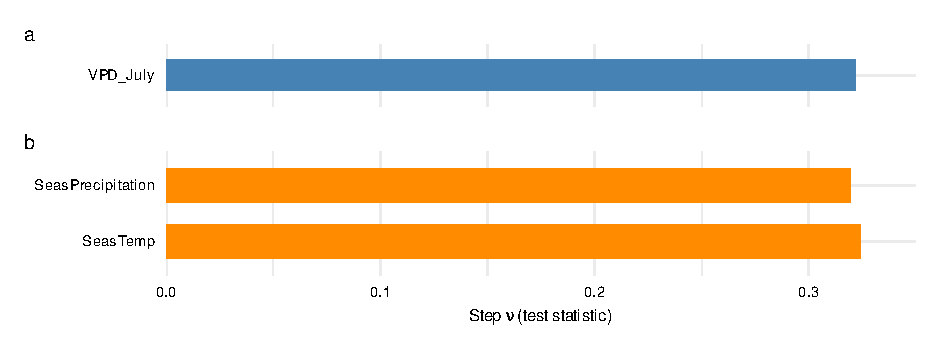
\includegraphics[width=\textwidth]{Fig6.pdf}
\caption{Variables selected by the FORD algorithm, (a) among the monthly climate variables and (b) among the seasonal aggregates. Bars show the test statistic (step $\nu$) at each selection step; variables are listed from top to bottom in the order of selection. Only variables with a statistically significant signal beyond random noise are retained: VPD in July for the monthly dataset, and seasonal precipitation followed by seasonal temperature for the seasonal dataset.}\label{fig:ford}
\end{figure}

\subsection{Machine learning predictive methods}

Across all dataset configurations and models, the predictive performance remained modest. Overall, only the tree-based ensemble methods (random forest, gradient boosting) outperformed the baseline model, but the improvement was moderate, while the LASSO did not beat the baseline (or only slightly).

\cref{fig:mae} summarises the model performance in terms of MAE across all models and configurations, including the baseline for reference; the corresponding detailed results are provided in \cref{tab:performance} in the Supplementary Material.

\begin{figure}[tbp]
\centering
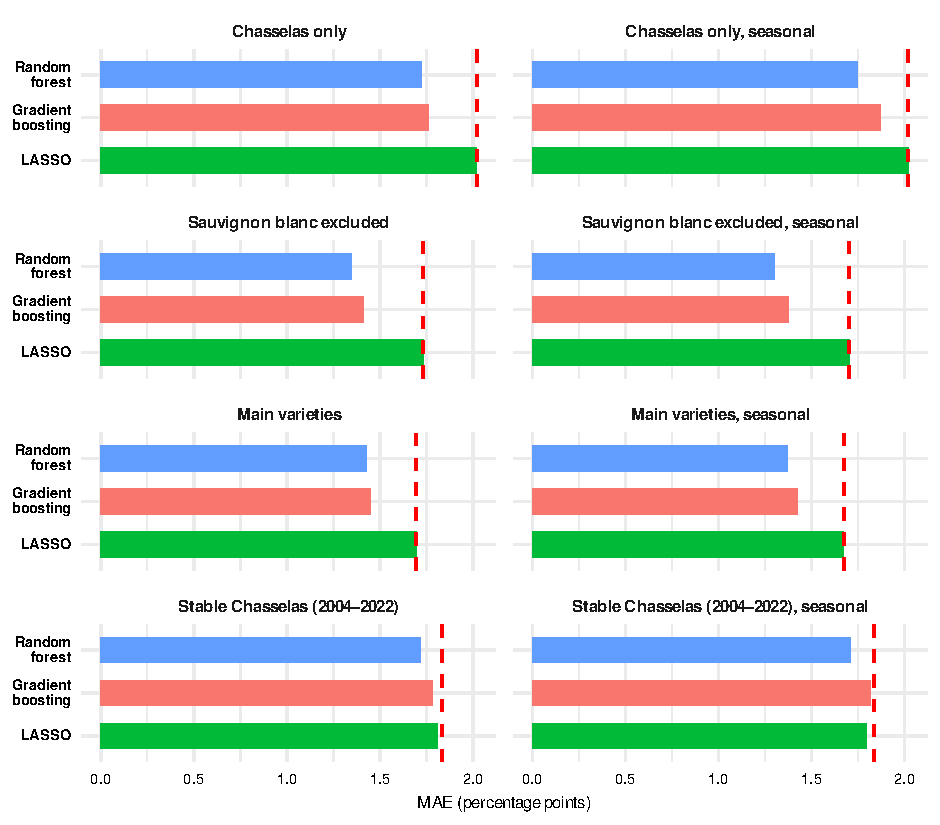
\includegraphics[width=\textwidth]{Fig7.pdf}
\caption{Test-set mean absolute error (MAE, in percentage points) of the three models (random forest, gradient boosting and LASSO) for each data configuration, using monthly climate variables (left) or seasonal aggregates (right). The dashed red vertical line is the baseline MAE (overall mean prediction); bars shorter than the baseline indicate better predictive performance.}\label{fig:mae}
\end{figure}

We can see that the major gain (23\% less of MAE compared to the baseline) is for the random forest trained on the whole dataset but the Sauvignon Blanc. We know that one plot with this variety has a particular history of unexplained susceptibility and is an outlier. The average incidence across all observations is approximately 2.56\% (median: 1.5\%), so a MAE of \textasciitilde1.5 (\% percents of incidence) represents a substantial error relative to the average observed incidence.

The best MAE are lower in all the configuration with more than a single cultivar (Exclude Sauvignon and Main varieties). Stable plots or chasselas only do not improve the performance of the models.

We can conclude that using a flexible tree-based model such as random forest and XGBoost improves upon a more interpretable model such as the LASSO. Other, more modern models such as tabPFN \citep{hollmann_accurate_2025} could potentially be used, but we do not expect dramatic improvement.

\subsection{Variable importance using predictive methods}

The combined variable importance analysis, summarized on \cref{fig:vimp}, revealed that the top-ranked variables were reasonably consistent across configurations:

\begin{itemize}
\tightlist
\item
  \textbf{VPD} (especially April, May, July, and the seasonal aggregate) was the most consistently top-ranked variable.
\item
  \textbf{Atmospheric pressure} (April--July) was prominent across configurations but showed more variability in ranking.
\item
  \textbf{Precipitation} (March--May) appeared in the top 10--15 across most configurations.
\end{itemize}

The ranking of variables beyond the top 3--5 varied substantially between configurations and models, suggesting limited stability. Relative humidity almost never appears as an important variable. This may be due to its effect being masked by VPD. Radiation also does not seem to affect the incidence of esca disease in any way.

The overall predictive performance remains modest (\cref{fig:mae}). This limits confidence in fine-grained variable importance distinctions. The results should be interpreted as identifying broad categories of potentially relevant climate drivers (VPD, atmospheric pressure, precipitation) rather than pinpointing specific variables with high confidence.

\begin{figure}[tbp]
\centering
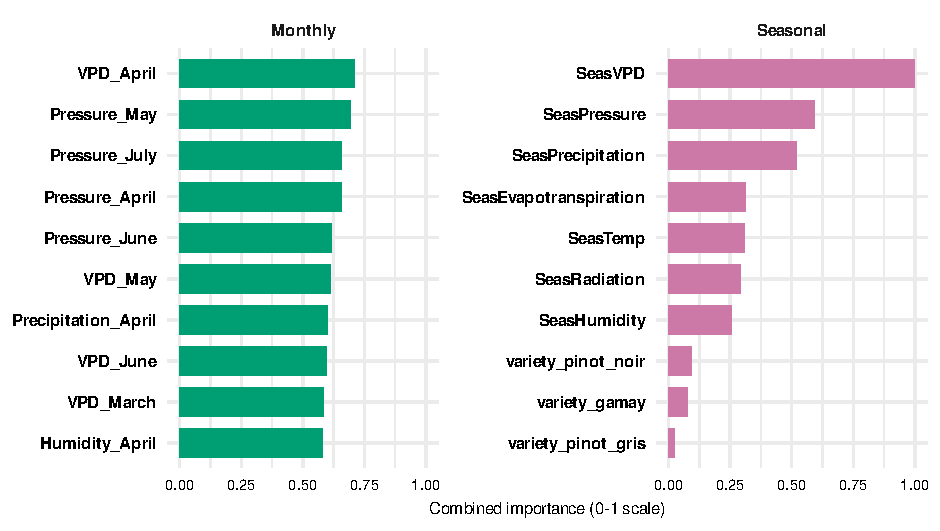
\includegraphics[width=\textwidth]{Fig8.pdf}
\caption{Combined variable importance (0--1 scale) of the ten most important variables, computed across all data configurations and models (random forest, gradient boosting, LASSO) and weighted by model performance, for the monthly (left) and seasonal (right) climate datasets.}\label{fig:vimp}
\end{figure}

\subsection{Regional comparison: rainfall/ET ratio and VPD versus esca incidence}

In addition to the predictive study, we sought to examine regional differences through comparisons of hydrometry. Since it has been shown that this factor is critical to the onset of symptoms \citep{bortolami_grapevines_2021,etienne_identification_2026}, we also sought to specifically examine this aspect at the regional level. The aim of this aggregation is to reveal a characteristic that is not discernible at plot level and that our predictive analysis fails to highlight. The P/ET ratios varied widely across regions and years, ranging from 0.5 to 2. To better capture the underlying trend, we used a smoothed median \citep{fasiolo_qgam_2021} which is less sensitive to outliers than a smooth mean.

As shown in Figure \ref{fig:regional}, higher P/ET ratios, reflecting wetter conditions relative to evaporative demand, and lower seasonal VPD, reflecting lower atmospheric dryness, were associated with higher median Esca incidence.

\begin{figure}[tbp]
\centering
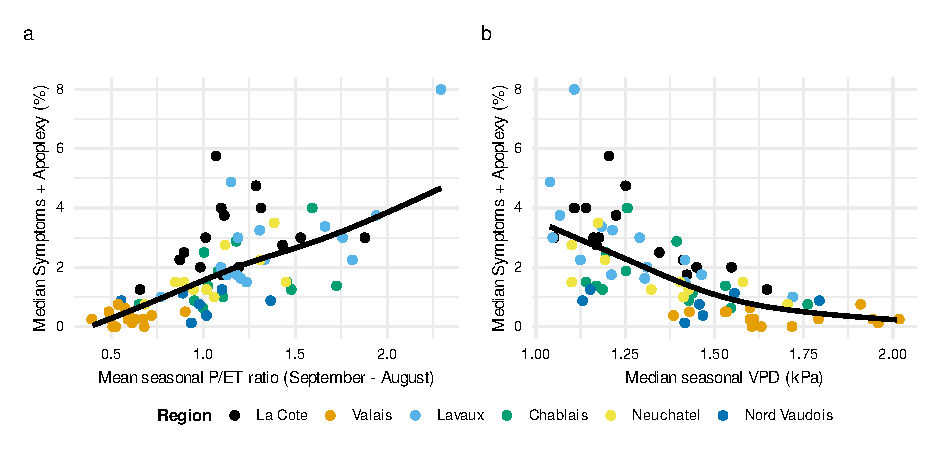
\includegraphics[width=\textwidth]{Fig9.pdf}
\caption{Relationship between esca incidence and climate for each region and year. Each point is a region--year pair; the y axis is the median incidence (\% of vine stocks with foliar symptoms or apoplexy) across the plots of the region. (a) Mean seasonal precipitation to evapotranspiration (P/ET) ratio, September--August; (b) median seasonal vapour pressure deficit (VPD, kPa). Colors indicate the region; the black line is a smooth median fitted to all points. Esca incidence increases with the P/ET ratio and decreases with VPD.}\label{fig:regional}
\end{figure}

Valais, the driest region (P/ET \textless{} 1, highest VPD), consistently shows the lowest Esca expression. Conversely, regions such as La Côte and Neuchâtel, which have higher P/ET ratios and lower VPD, show higher Esca expression.
